% Adjust these for the path of the theme and its graphics, relative to this file
%\usepackage{beamerthemeFalmouthGamesAcademy}
\usepackage{../../beamerthemeFalmouthGamesAcademy}
\usepackage{multimedia}
\graphicspath{ {../../} }

% Default language for code listings
\lstset{language=C++,
        morekeywords={each,in,nullptr}
}

% From http://blog.virtualglobebook.com/2011/02/syntax-highlighting-c-and-glsl-source.html

\lstdefinelanguage{GLSL}
{
sensitive=true,
morekeywords=[1]{
attribute, const, uniform, varying,
layout, centroid, flat, smooth,
noperspective, break, continue, do,
for, while, switch, case, default, if,
else, in, out, inout, float, int, void,
bool, true, false, invariant, discard,
return, mat2, mat3, mat4, mat2x2, mat2x3,
mat2x4, mat3x2, mat3x3, mat3x4, mat4x2,
mat4x3, mat4x4, vec2, vec3, vec4, ivec2,
ivec3, ivec4, bvec2, bvec3, bvec4, uint,
uvec2, uvec3, uvec4, lowp, mediump, highp,
precision, sampler1D, sampler2D, sampler3D,
samplerCube, sampler1DShadow,
sampler2DShadow, samplerCubeShadow,
sampler1DArray, sampler2DArray,
sampler1DArrayShadow, sampler2DArrayShadow,
isampler1D, isampler2D, isampler3D,
isamplerCube, isampler1DArray,
isampler2DArray, usampler1D, usampler2D,
usampler3D, usamplerCube, usampler1DArray,
usampler2DArray, sampler2DRect,
sampler2DRectShadow, isampler2DRect,
usampler2DRect, samplerBuffer,
isamplerBuffer, usamplerBuffer, sampler2DMS,
isampler2DMS, usampler2DMS,
sampler2DMSArray, isampler2DMSArray,
usampler2DMSArray, struct},
morekeywords=[2]{
radians,degrees,sin,cos,tan,asin,acos,atan,
atan,sinh,cosh,tanh,asinh,acosh,atanh,pow,
exp,log,exp2,log2,sqrt,inversesqrt,abs,sign,
floor,trunc,round,roundEven,ceil,fract,mod,modf,
min,max,clamp,mix,step,smoothstep,isnan,isinf,
floatBitsToInt,floatBitsToUint,intBitsToFloat,
uintBitsToFloat,length,distance,dot,cross,
normalize,faceforward,reflect,refract,
matrixCompMult,outerProduct,transpose,
determinant,inverse,lessThan,lessThanEqual,
greaterThan,greaterThanEqual,equal,notEqual,
any,all,not,textureSize,texture,textureProj,
textureLod,textureOffset,texelFetch,
texelFetchOffset,textureProjOffset,
textureLodOffset,textureProjLod,
textureProjLodOffset,textureGrad,
textureGradOffset,textureProjGrad,
textureProjGradOffset,texture1D,texture1DProj,
texture1DProjLod,texture2D,texture2DProj,
texture2DLod,texture2DProjLod,texture3D,
texture3DProj,texture3DLod,texture3DProjLod,
textureCube,textureCubeLod,shadow1D,shadow2D,
shadow1DProj,shadow2DProj,shadow1DLod,
shadow2DLod,shadow1DProjLod,shadow2DProjLod,
dFdx,dFdy,fwidth,noise1,noise2,noise3,noise4,
EmitVertex,EndPrimitive},
morekeywords=[3]{
gl_VertexID,gl_InstanceID,gl_Position,
gl_PointSize,gl_ClipDistance,gl_PerVertex,
gl_Layer,gl_ClipVertex,gl_FragCoord,
gl_FrontFacing,gl_ClipDistance,gl_FragColor,
gl_FragData,gl_MaxDrawBuffers,gl_FragDepth,
gl_PointCoord,gl_PrimitiveID,
gl_MaxVertexAttribs,gl_MaxVertexUniformComponents,
gl_MaxVaryingFloats,gl_MaxVaryingComponents,
gl_MaxVertexOutputComponents,
gl_MaxGeometryInputComponents,
gl_MaxGeometryOutputComponents,
gl_MaxFragmentInputComponents,
gl_MaxVertexTextureImageUnits,
gl_MaxCombinedTextureImageUnits,
gl_MaxTextureImageUnits,
gl_MaxFragmentUniformComponents,
gl_MaxDrawBuffers,gl_MaxClipDistances,
gl_MaxGeometryTextureImageUnits,
gl_MaxGeometryOutputVertices,
gl_MaxGeometryOutputVertices,
gl_MaxGeometryTotalOutputComponents,
gl_MaxGeometryUniformComponents,
gl_MaxGeometryVaryingComponents,gl_DepthRange},
morecomment=[l]{//},
morecomment=[s]{/*}{*/},
morecomment=[l][keywordstyle4]{\#},
}


% For strikethrough effect
\usepackage[normalem]{ulem}
\usepackage{wasysym}

\usepackage{pdfpages}

\usepackage{caption}
\captionsetup[figure]{font=scriptsize,labelfont=scriptsize}

% http://www.texample.net/tikz/examples/state-machine/
\usetikzlibrary{arrows,automata}

\newcommand{\modulecode}{COMP260}\newcommand{\moduletitle}{Distributed Systems}\newcommand{\sessionnumber}{5}

\begin{document}
\title{\sessionnumber: Post-Processing}
\subtitle{\modulecode: \moduletitle}

\frame{\titlepage} 

\begin{frame}{Learning outcomes}
	By the end of this week, you should be able to:
	\begin{itemize}
		\item \textbf{Recall} alternative ways to represent mesh vertices in memory.
		\item \textbf{Apply} basic transforms using the GLM library.
		\item \textbf{Explain} the constituents of the model-view-projection matrix and how it can be used to create a first-person camera controller.
	\end{itemize}
\end{frame}

\begin{frame}{Agenda}
	\begin{itemize}
		\pause\item Lecture (async):
		\begin{itemize}
			\item \textbf{Compare} different ways to store vertex data in memory.
			\item \textbf{Review} the transforms required to display 3D objects on a 2D screen.
		\end{itemize}
		\pause\item Workshop (sync):
		\begin{itemize}
			\item \textbf{Adapt} our basic triangle implementation to draw meshes with multiple triangles efficiently.
			\item \textbf{Experiment} with creating transforms using GLM and using them to move objects and the camera.
		\end{itemize}
	\end{itemize}
\end{frame}

\part{Post-processing}
\frame{\partpage}

\begin{frame}{What is Post-Processing?}
	\begin{itemize}
		\pause\item A series of techniques that are carried out \textbf{after} a scene has been rendered
		\pause\item Typically mimic effects caused by camera (or eye) hardware, e.g. lens flare, bloom, motion blur
		\pause\item Traditionally this could only be done as an offline process
		\pause\item With the advent of faster GPUs and programmable shaders, we can implement some of the effects in real time
	\end{itemize}
\end{frame}

\begin{frame}{Post-Processing Stages}
	\begin{itemize}
		\pause\item The key to the effect is to switch from drawing to the back buffer to a \textbf{texture}
		\pause\item This texture will contain the current view of the scene
		\pause\item We then use a shader to implement a post-processing effect
		\pause\item We then map the processed texture onto a full screen quad, which is rendered to the backbuffer
	\end{itemize}
\end{frame}

\begin{frame}{The Frame Buffer}
	\begin{itemize}
		\pause\item We use several types of \textbf{screen buffers} when rendering with OpenGL:
		\begin{itemize}
			\pause\item The \textbf{colour buffer} stores the pixel output from the fragment shaders.
			\pause\item The \textbf{depth buffer} (or $z$-buffer) stores information for depth-testing.
			\pause\item A \textbf{stencil buffer} can be used to mask out certain fragments.
		\end{itemize}
		\pause\item A \textbf{framebuffer} is just a combination of different buffers.
		\pause\item A default framebuffer is created for you; you can create additional ones to render to instead.
	\end{itemize}
\end{frame}
\part{COMP120 Refresher}
\frame{\partpage}

\begin{frame}{Image Processing Techniques}
	\begin{itemize}
		\item\pause Some of the algorithms you learned in COMP120 can be applied in GLSL:
		\begin{itemize}
			\item Colour Replacement
			\item Luminance calculation  
			\item Colour Correction
			\item Black \& White and Sepia Tone
			\item Edge Detection
		\end{itemize}
		\pause\item Key difference: we access the data via \textbf{texture coordinates}, rather than array indices.
	\end{itemize}
\end{frame}

\begin{frame}{Modifying Textures}
	\begin{itemize}
		\item\pause A Texture Lookup uses the texture coordinates passed to the fragment shader
		\item\pause Additionally, the fragment shader only processes a single fragment at a time
		\item\pause If we want to access a pixel adjacent to the current one, we can offset the current texture coordinates - this is especially useful for edge detection
		\item\pause GLSL has lots of inbuilt functions (e.g distance) which can aid in creating post-processing effects
	\end{itemize}
\end{frame}
\part{Other Post Processing Techniques}
\frame{\partpage}

  \begin{frame}
	\frametitle{Colour Correction}
	\begin{columns}
		\begin{column}{0.5\textwidth}
			\begin{itemize}
				\item Process of taking an image, convert each colour in the image to a some other colour
				\item Mimic a specific film stock, provide coherent look or provide a mood
			\end{itemize}
		\end{column}
		\begin{column}{0.5\textwidth}
			\begin{center}
				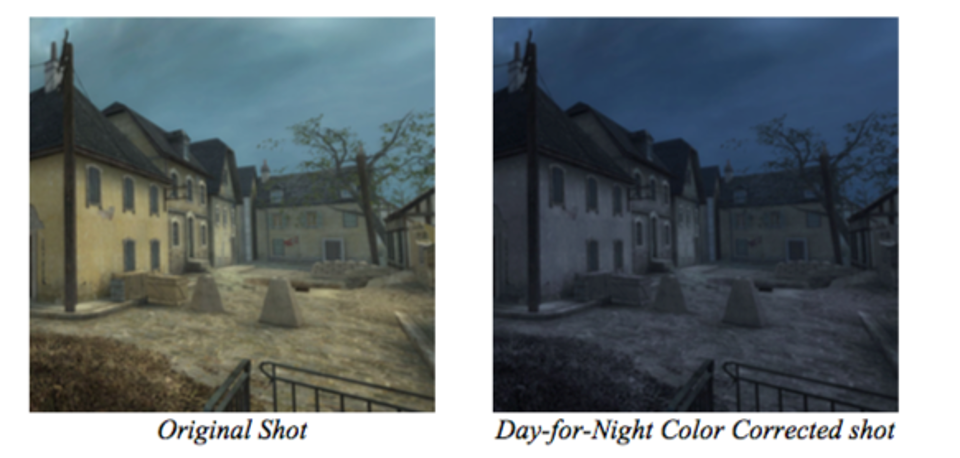
\includegraphics[width=\textwidth]{colour_correction_daynight}
			\end{center}
		\end{column}
	\end{columns}
\end{frame}


\begin{frame}
	\frametitle{Colour Correction Again}
		\begin{columns}
		\begin{column}{0.5\textwidth}
			\begin{itemize}
				\item Depending on the technique this could involve manipulating the colours using a Filter Kernel
				\item Or we could use a colour palette (see Colour Grading) 
			\end{itemize}
		\end{column}
		\begin{column}{0.5\textwidth} 
			\begin{center}
				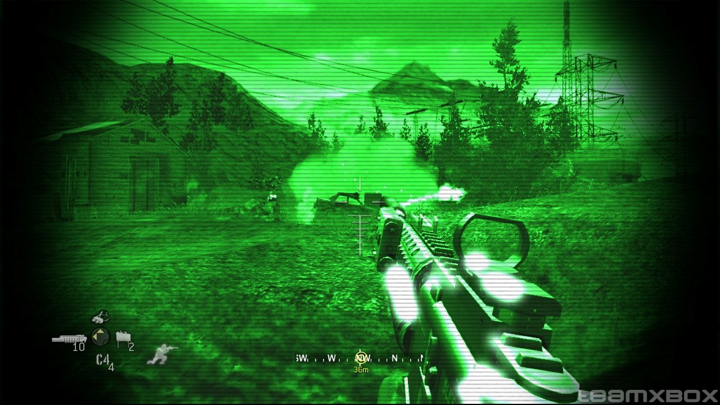
\includegraphics[width=\textwidth]{colour_correction_nightvision}
			\end{center}
		\end{column}
	\end{columns}
\end{frame}

\begin{frame}{Blur}
	\begin{itemize}
		\item\pause This often used as a basis for other techniques such as Depth of Field and HDR
		\item\pause To achieve blurring we apply a filter to the texture lookup of the texture render target
		\item\pause We can apply many different filters, one of the simplest is a Box Filter
		\item\pause With a box filter we sample 4 points around the point we are interested in
	\end{itemize}
\end{frame}

\begin{frame}
	\frametitle{Motion Blur}
\begin{columns}
	\begin{column}{0.5\textwidth}
		\begin{itemize}
			\item If an object moves very fast through you Field of view it can appear that the object leaves a slight ghost of itself
			\item There are several ways of implementing this, we can use the actual speed of the object to determine the amount of blur
		\end{itemize}
	\end{column}
	\begin{column}{0.5\textwidth} 
		\begin{center}
			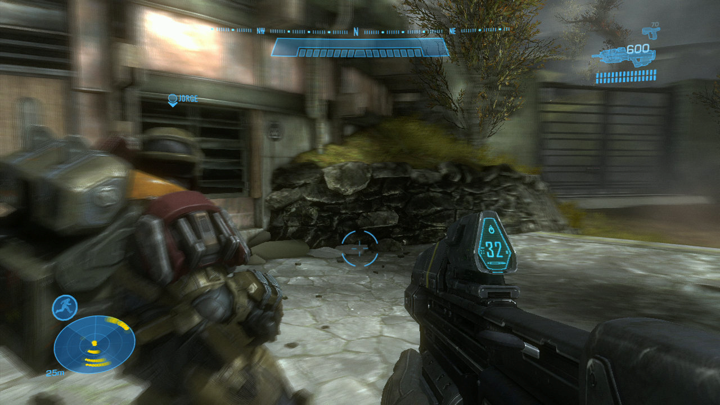
\includegraphics[width=\textwidth]{motion_blur}
		\end{center}
	\end{column}
\end{columns}
\end{frame}

\begin{frame}
	\frametitle{Motion Blur}
	\begin{columns}
		\begin{column}{0.5\textwidth}
			\begin{itemize}
				\item Or we can simply take the results of the last render update and blend them with current render results and blend based on a lerp
			\end{itemize}
		\end{column}
		\begin{column}{0.5\textwidth} 
			\begin{center}
				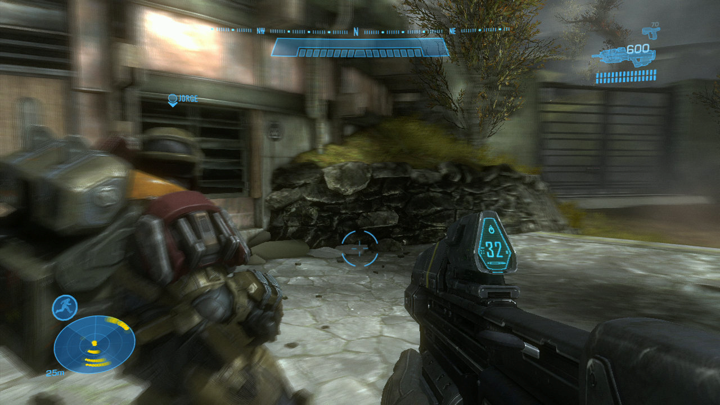
\includegraphics[width=\textwidth]{motion_blur}
			\end{center}
		\end{column}
	\end{columns}
\end{frame}

\begin{frame}
	\frametitle{Depth of Field}
\begin{columns}
	\begin{column}{0.5\textwidth}
		\begin{itemize}
			\item DOF attempts to simulate the effect where object that are too close or too far away appear out of focus
			\item We first have to consider in our scene what range of depth values will be considered in focus. We then need to blur everything that is outside this range
		\end{itemize}
	\end{column}
	\begin{column}{0.5\textwidth} 
		\begin{center}
			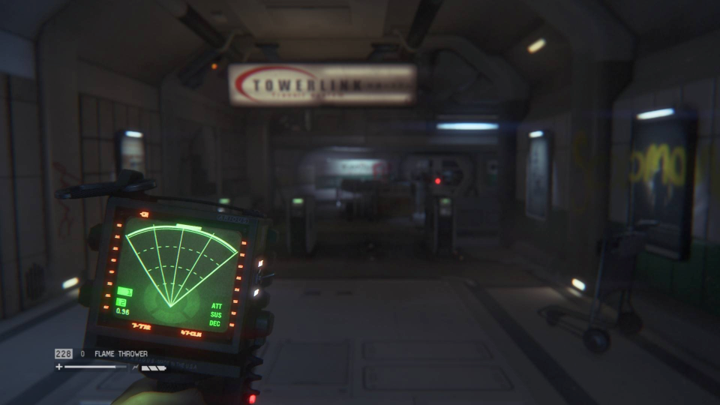
\includegraphics[width=\textwidth]{depth_of_field}
		\end{center}
	\end{column}
\end{columns}	
\end{frame}

\begin{frame}
	\frametitle{Depth of Field}
	\begin{columns}
		\begin{column}{0.5\textwidth}
			\begin{itemize}
				\item Once we have determined this we render a blurred scene to a render texture
			\end{itemize}
		\end{column}
		\begin{column}{0.5\textwidth} 
			\begin{center}
				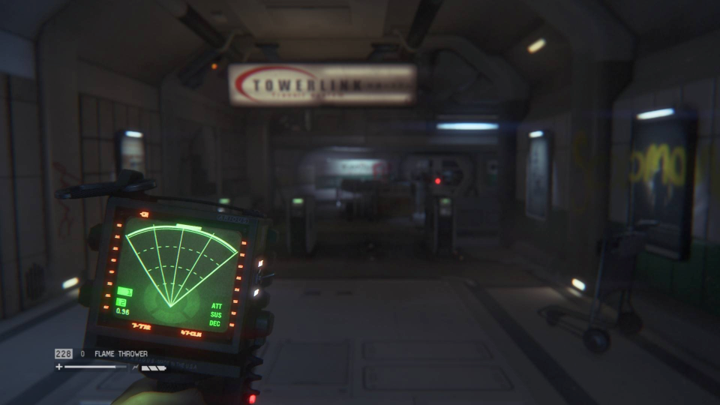
\includegraphics[width=\textwidth]{depth_of_field}
			\end{center}
		\end{column}
	\end{columns}	
\end{frame}

\begin{frame}
	\frametitle{Bloom}
	\begin{columns}
		\begin{column}{0.5\textwidth}
			\begin{itemize}
				\item This attempts to simulate the overloading of the optic nerve if extremely bright areas of a surface are visible
				\item First of we render to a smaller render target usually 1/4 size
			\end{itemize}
		\end{column}
		\begin{column}{0.5\textwidth} 
			\begin{center}
				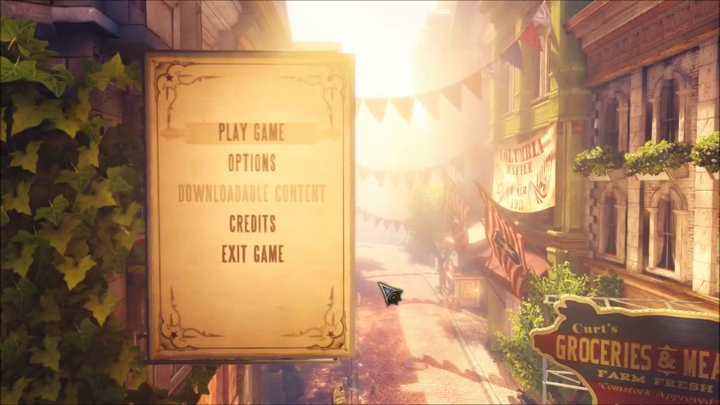
\includegraphics[width=\textwidth]{bloom}
			\end{center}
		\end{column}
	\end{columns}	
\end{frame}

\begin{frame}
	\frametitle{Bloom}
	\begin{columns}
		\begin{column}{0.5\textwidth}
			\begin{itemize}
				\item We then apply a filter(usually Gauss) to this reduced render target, if we apply this filter of multiple passes then we achieve a smoother blur
				\item We then blend the blurred image onto the screen with the original scene 
			\end{itemize}
		\end{column}
		\begin{column}{0.5\textwidth} 
			\begin{center}
				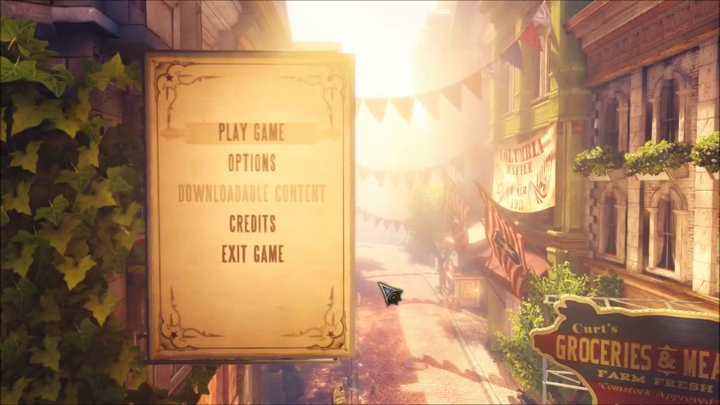
\includegraphics[width=\textwidth]{bloom}
			\end{center}
		\end{column}
	\end{columns}	
\end{frame}

\begin{frame}{Next steps}
	\begin{itemize}
		\item \textbf{Review} the additional asynchronous material for more background on the framebuffer and various post-processing (or image processing) effects.
		\item \textbf{Attend} the workshop to learn how to save a rendered scene to a texture in OpenGL and apply effects to it in a shader.
	\end{itemize}
\end{frame}

\end{document}

